\documentclass{article}

\usepackage{graphicx}
\usepackage{hyperref}
\usepackage{listings}
\usepackage{color}
\usepackage{verbatim}
%\usepackage{subfigure}
\usepackage{amsmath}
\usepackage{caption}
\usepackage{subcaption}
\usepackage{placeins}
\usepackage{setspace}

\linespread{1.5}

\begin{document}

\section{Results}
\subsection{Graphs}
We have a set of graphs that are similar to the power-law graphs from Watts-Strogatz and Chung-Lu \cite{Watts:1998,Chung:2004}. These encompass a wide range of subjects from biological processes, social networks, and urban infrastructure. To standardize the datasets, I coerced them into undirected, unweighted networks, however I can solve a similar linear system if they are in their original form. In addition to a short description of the datasets and what it means to solve their Laplacian linear system, I created a spy plot of the Laplacian matrix, a degree histogram, a simple network graphic to illustrate connections in the data, and a plot of the singular values of $T_L$ to show its low-rank structure.
\subsubsection{\textit{C. Elegans} Worm Data}
The \textit{C. Elegans} worm has been studied extensively due to the low complexity of it's biological systems. The smallest graph in this results section is the completely mapped nervous system of 297 neurons in the worm with 2148 connections from initial experimental data given by White et. al. in 1986 \cite{White:1986,Watts:1998}. Solving the Laplacian linear system of a neural network is analogous to finding the PageRank vector of  influences for each neuron. The neural edge information can be combined with anatomical information about brain regions to study which parts of the brain are more important for different functions. Another possible study identifies how an organism's brain of an organism develops as it ages \cite{Gleich:2015}.

\begin{figure}
\centering

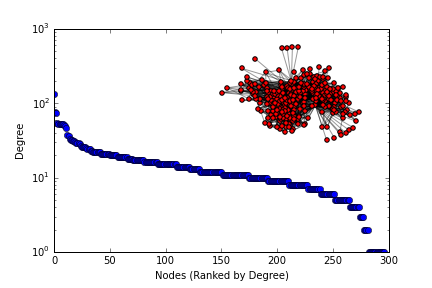
\includegraphics[width=\linewidth]{neural_degree_histogram.png}
\caption{Neural Network of \textit{C. Elegans}}
  
\end{figure}

\begin{figure}
\centering
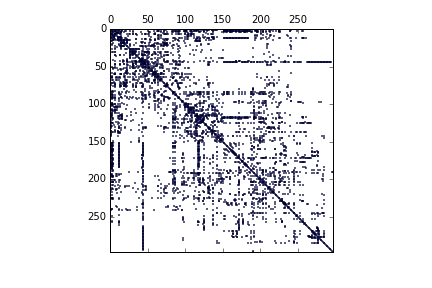
\includegraphics[width = \linewidth]{neuralspy.png}
\caption{Spy Plot of Neural Network Laplacian Matrix}
\end{figure}
\begin{figure}
\centering
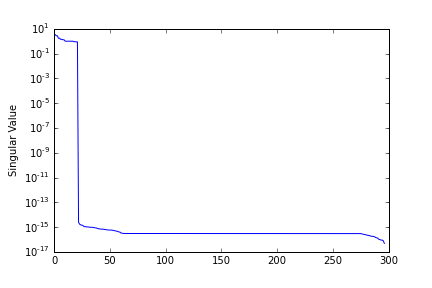
\includegraphics[width = \linewidth]{neuralsing.png}
\end{figure}

The second \textit{C. Elegans} dataset describes the 453 metabolic processes and their 2025 connections that comprise the metabolism of the worm \cite{Duch:2005}. Again, this is a simple network of a simple organism. Solving the Laplacian linear system can offer insights into the key metabolic processes.

\begin{figure}
\centering

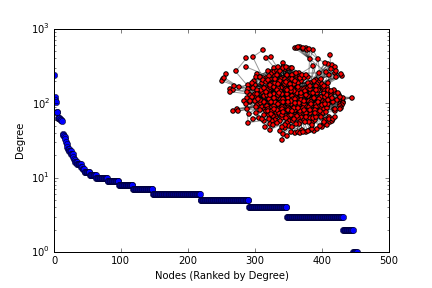
\includegraphics[width=\linewidth]{meta_degree_histogram.png}
\caption{Metabolic Network of \textit{C. Elegans}}
  
\end{figure}
\begin{figure}
\centering
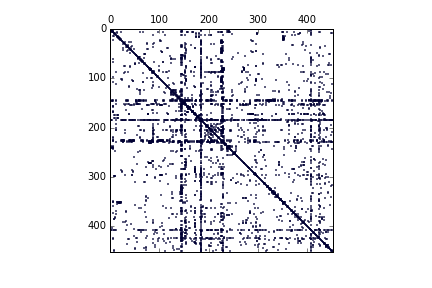
\includegraphics[width = \linewidth]{metaspy.png}
\caption{Spy Plot of Metabolic Network Laplacian Matrix}
\end{figure}
\begin{figure}
\centering
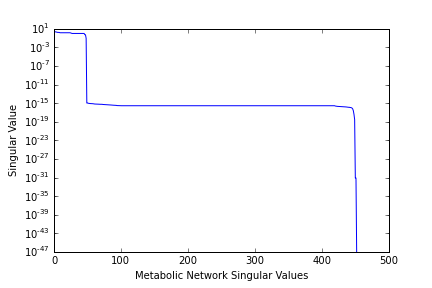
\includegraphics[width = \linewidth]{metasing.png}
\end{figure}


The final \textit{C. Elegans} dataset is an order of magnitude larger than the previous two. The worm's genetics encode proteins that ultimately display phenotypes. Networks of this type are described as interactomes. The graph I study has 912 proteins with 22,738 edges for protein-protein interactions with corresponding, scientifically-observed phenotypes \cite{Simonis:2009}. Solving the Laplacian linear system for a protein network can highlight unobserved, tangential protein-phenotype relationships \cite{Gleich:2015}.

\begin{figure}
\centering

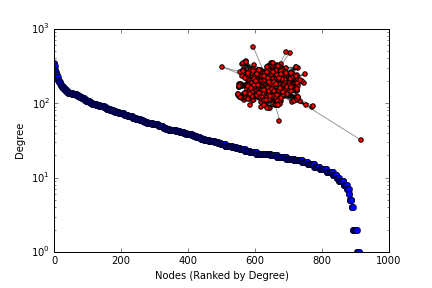
\includegraphics[width=\linewidth]{gene_degree_histogram.png}
\caption{Protein Network with Corresponding Phenotypes of \textit{C. Elegans}}
  
\end{figure}

\begin{figure}
\centering
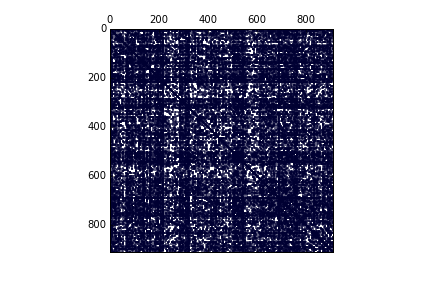
\includegraphics[width = \linewidth]{genespy.png}
\caption{Spy Plot of Protein Network Laplacian Matrix}
\end{figure}
\begin{figure}
\centering
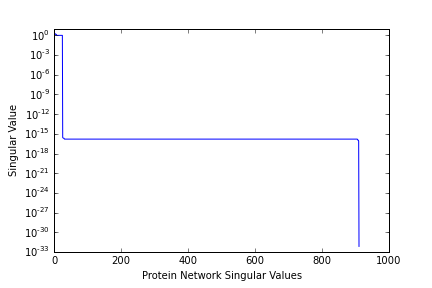
\includegraphics[width = \linewidth]{proteinsing.png}
\end{figure}

While the \textit{C. Elegans} worm is an incredibly, biologically simple organism, it is useful as a test case for solving much larger linear systems for more complex organisms. The ultimate goal, of course, to map the biological systems of humans. Already, work is being done to map the human interactome \cite{Rual:2005,Rolland:2014} and parts of the human neural network \cite{Toga:2012}. All three of the worm networks are comprised of a highly locally-connected subgraph and small teleportation subgraph making them amenable to my method. 

\subsubsection{Facebook Friend Circles}
The largest graph I work with contains the 88,234 Facebook friend connections between 4039 users  \cite{Mcauley:2012}. Social scientists are interested in identifying sources of influence in a social network. By solving the Laplacian linear system associated with the Facebook graph I can solve a so-called "reverse" PageRank system. This finds the origins of influence; for a circle of Facebook friends, it might identify how those people became connected through a few key people. This can be applied to any network of human interactions including other social networks, or organizational systems \cite{Gleich:2015}. This graph is also highly locally-connected, and is a good example of how my method scales to larger networks.

\begin{figure}
\centering

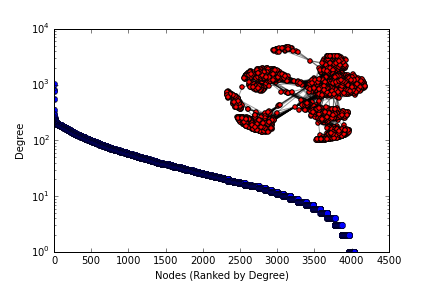
\includegraphics[width=\linewidth]{fb_degree_histogram.png}
\caption{Facebook Friend Network}
  
\end{figure}

\begin{figure}
\centering
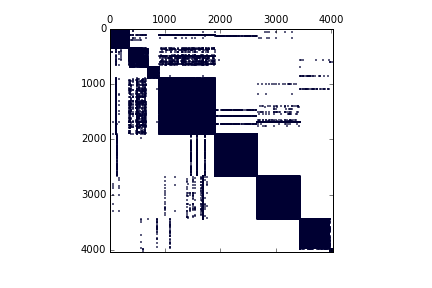
\includegraphics[width = \linewidth]{fbspy.png}
\caption{Spy Plot of Facebook Network Laplacian Matrix}
\end{figure}
\begin{figure}
\centering
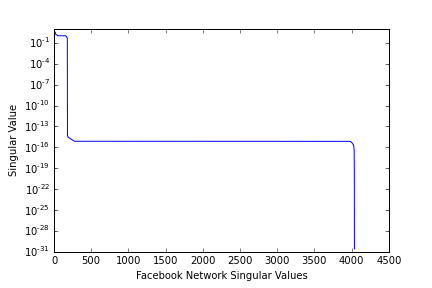
\includegraphics[width = \linewidth]{fbsing.png}
\end{figure}

\subsubsection{Western US Power Grid}
The final dataset illustrates how my method fails. The Western US power grid has 4941 nodes and 6594 connections \cite{Watts:1998}; this is a much lower edge/node ratio than the previous datasets and explains why this graph is not very locally-connected. Whereas the previous 4 examples resulted in low-rank teleportation laplacian matrix, $T_L$ for the power grid is almost full-rank. As seen further, the resulting linear system solve requires way too many floating point operations. Solving this system can describe the flow of electricity through the grid \cite{Pagani:2013}, however my method clearly is not appropriate. 

\begin{figure}
\centering

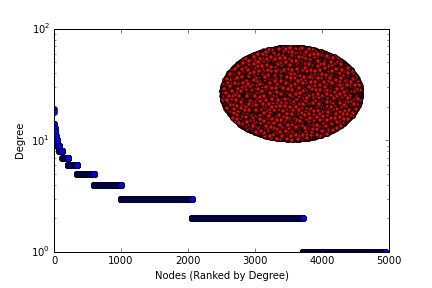
\includegraphics[width=\linewidth]{power_degree_histogram.png}
\caption{Network of Western Power Grid}
  
\end{figure}

\begin{figure}
\centering
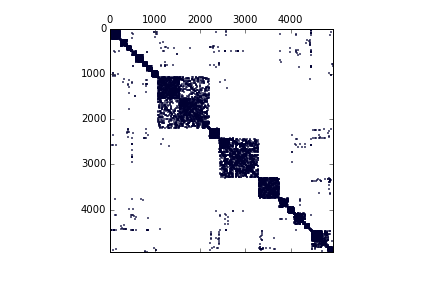
\includegraphics[width = \linewidth]{powerspy.png}
\caption{Spy Plot of Power Grid Laplacian Matrix}
\end{figure}

\begin{figure}
\centering
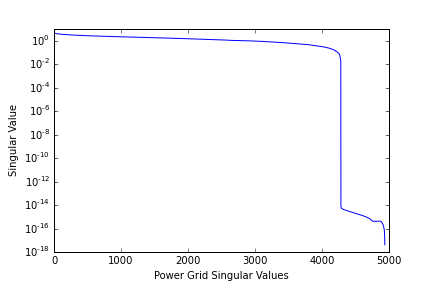
\includegraphics[width = \linewidth]{powersing.png}
\end{figure}

\subsubsection{Graph Overview}
The key part of my algorithm is partitioning a graph into a large locally-connected subgraph and a small teleportation subgraph. Four of these examples fully fit into this class of graphs, whereas the power grid most certainly does not as evidenced below. The important attribute to look for is low rank of the teleportation Laplacian matrix relative to the number of the nodes (which is the size of the entire square Laplacian matrix). Here is a table summarizing the datasets:

\begin{spacing}{1}
\begin{center}
\renewcommand{\arraystretch}{1.5}
    \begin{tabular}{| l | l | l |}
    \hline
    Graph (nodes, edges) & Rank $T_L$ & Rank/nodes \\ \hline
    Neural (297, 2148) & 22 & .0741 \\ \hline
    Metabolic (453, 2025) & 49 & .1082 \\  \hline
    Protein (912, 22738) & 26 & .0285 \\ \hline
    Facebook (4039, 88234) & 180 & .0446 \\ \hline
    Power (4941, 6594) & 4284 & .8670 \\ 
    \hline
    \end{tabular}
\end{center}
\end{spacing}

\subsection{Graph Partitioning}
Partitioning the complete graph into the maximum locally-connected subgraph and the teleportation graph is the unique part of this algorithm. This requires an initial computational step as an overhead cost. Any graph must only be partitioned once, as the unique edgelists can be written into files for future use. In the methodology section I mentioned that that each graph follows a power-law degree distribution with $2 < \gamma < 3$ which affects its expected degree. However, for finite node graphs, $\gamma$ can be less than 2 and the degree sequence decay is stretched. Let's take a look at the degree histrogram for the \textit{C. Elegans} neural network compared to a typical power-law degree distribution and a stretched power-law distribution:

\begin{figure}
\centering
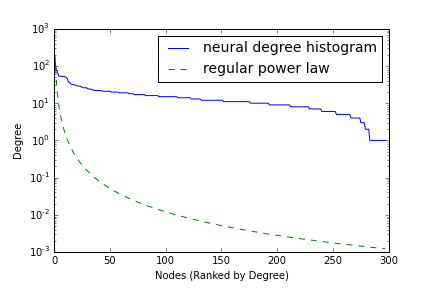
\includegraphics[width = \linewidth]{neuralsequenceplot2.png}
\caption{Degree sequences of Neural Network and standard power law distribution ($\gamma = 2.1$)}
\end{figure}

\begin{figure}
\centering
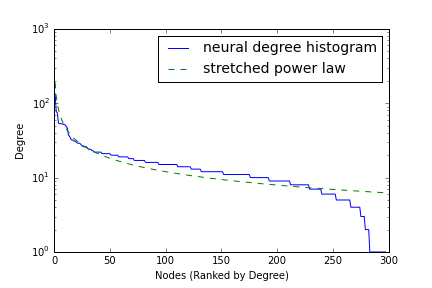
\includegraphics[width = \linewidth]{neuralsequenceplot.png}
\caption{Degree sequences of Neural Network and stretched power law distribution ($\gamma = .6$ in numerator)}
\end{figure}

Clearly the stretched power-law distribution fits the data better. The finite node power-law distribution has $E[d] \approx 1$, the stretched power-law distribution has $E[d] = 14.39$ and the average degree of the neural network is 14.46. This matters because it affects the complexity of the partitioning algorithm which has $O(iter.\times m\times (E[d]^3))$. I want to more accurately predict the computational cost of the partitioning algorithm.

\subsubsection{Table of Partitioning results} 
\begin{spacing}{1}
\begin{center}
\renewcommand{\arraystretch}{1.5}
    \begin{tabular}{| l | l | l | l | l |}
    \hline
    Graph ($V$, $E$) & Avg. Deg. & Nx Part. (s) & Part. (s) & $N_I$ \\ \hline
    Neural (297, 2148) & 14.46 & 11 & 1.6 & 3 \\ \hline
    Metabolic (453, 2025) & 8.94 & 12 & 2.3 & 3 \\  \hline
    Protein (912, 22738) & 49.86 & 1915 & 53 & 2 \\ \hline
    Facebook (4039, 88234) & 43.69 & 11593 & 480 & 3 \\ \hline
    Power (4941, 6594) & 2.669 & 2.1 & .33 & 3 \\ 
    \hline
    \end{tabular}
\end{center}
\end{spacing}

\begin{figure}
\centering
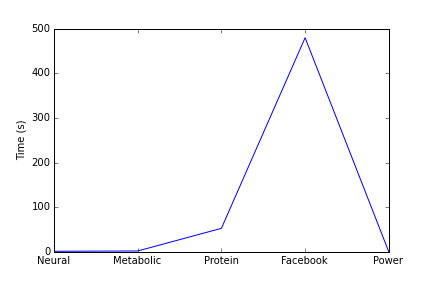
\includegraphics[width = \linewidth]{ptimes.png}
\caption{Partitioning graph times. Note how the time increases by the third power for the first four. The Partitioning drops for the power grid with low average degree.}
\end{figure}

The partitioning times are in line with the theoretical complexity except for the metabolic network which has a similar number of edges but lower average degree than the neural network, and takes longer to partition. I hypothesize that because the graph is double the size, there is an additional overhead to using the NetworkX functions to create pathways and loop through all possible edges. I add the NetworkX partitioning times (Nx Part. (s)) to show how much more computation the NetworkX partitioning requires with the shortest path algorithm. Granted, searching through increasing path lengths requires exponentially more work, so this is probably infeasible for increasing $k$ beyond 5. In addition I show the number of iterations of edge deletion, $N_I$, until the maximum locally-connected subgraph is recovered.

\subsection{Linear System Solve}
I want to dig deeper into the solve portion to determine if the operations correspond with their given theoretical complexities. Here is a table of the timings for the individual operations:\\
\begin{spacing}{1}
\begin{center}
\renewcommand{\arraystretch}{1.5}
    \begin{tabular}{ | l | l | l | l | l | l | l |}
    \hline
    \textbf{Operation} & \textbf{$O(r,n)$} & \textbf{Neur.} & \textbf{Meta.} & \textbf{Prot.} & \textbf{FB} & \textbf{Pow.} \\ \hline
    $USV = T_L$ & $O(n^3)$ & .0334 & .0737 & .4183 & 38.47 & 72.86  \\ \hline
    $S^{-1}$ & $O(r)$ & .0005 & .0007 & .0001 & .0023 & 5.104 \\ \hline
    $y = P_L^{-1}b$ (MG) & $O(n)$ & .0857 & .0962 & .3552 & 1.347 & .1152  \\  \hline
    $y_1 = Vy$ & $O(rn)$ & .0013 & .0015 & .0002 & .0023 & .0702 \\ \hline
    $Q = P_L^{-1}U$ ($r\times$MG) & $O(rn)$ & .3292 & .7360 & .5190 & 23.11 & 106.9  \\ \hline
    $Q_1 = VQ$ & $O(r^2 n)$ & .0006 & .0036 & .0013 & .4124 & 285.1 \\ \hline
    $Q_2 = S^{-1} + Q_1$ & $O(r^2)$ & .0012 & .0018 & .0003 & .0011 & .4157 \\ \hline
    $y_2 = Q_2^{-1}y_1$ & $O(r^3)$ & .0023 & .0025 & .0013 & .0099 & 86.49 \\ \hline
    $y_3 = Uy_2$ & $O(rn)$ & .0001 & .0002 & .0003 & .0025 & .1867 \\ \hline
    $y_4 = P_L^{-1}y_3$ (MG) & $O(n)$ &.0128 & .0070 & .1183 & .8249 & .0059 \\ \hline
    $x = y - y_4$ & $O(n)$ &.0003 & .0003 & .0003 & .0004 & .0003 \\ \hline
    \textbf{Total} & \textbf{$O(n^3)$} & \textbf{.51} & \textbf{.966} & \textbf{1.44} & \textbf{64.46} & \textbf{560} \\
    \hline
    \end{tabular}
\end{center}
\end{spacing}
\begin{figure}
\centering
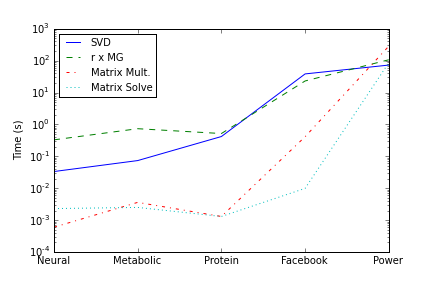
\includegraphics[width = \linewidth]{operationtimes.png}
\caption{Solve times for the limiting operations. Note: does not scale for full-rank power grid graph}
\end{figure}

\begin{figure}
\centering
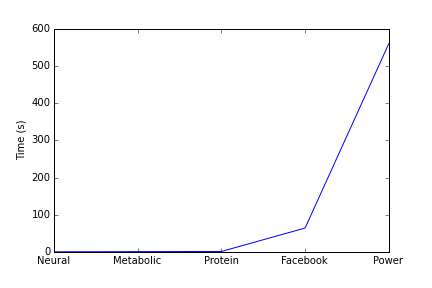
\includegraphics[width = \linewidth]{stimes.png}
\caption{Linear system solve times.}
\end{figure}

For the first four examples (not including the power grid solve), the limiting operations are the singular value decomposition and multiple right hand side multigrid solves, $Q = P_L^{-1}U$. 
\subsubsection{SVD and Multiple Multigrid Solves}
The SVD is an efficient operation that allows for peak performance (work done per data input) \cite{Berry:2006}. Thus it is beneficial to have this as a limiting operation. There are alternative algorithms for computing the SVD such as an analogous method to randomized QR \cite{Halko:2011} that are faster. In addition, it is possible to utilize the low-rank structure of $T_L$ to further decrease computation. It is also ideal to be constrained by a multiple right-hand-side multigrid solve step. By vectorizing the multiple right-hand-sides I can achieve more computational work per multigrid solve. This combined with low-rank aspect will greatly speed up the overall solve routine.
\subsubsection{Power Grid}
However for the full rank power-grid solve, the limiting operations are the SVD, the matrix-matrix multiplication, $Q_1 = VQ$, and the matrix solve, $y_2 = Q_2^{-1}y_1$. The latter two cannot be optimized for dense matrices, and will not scale well for larger graphs without the low-rank structure of the teleportation subgraph Laplacian matrix. Thus graphs with low average degree, large $V$, and lacking a large locally-connected portion should not be used for solving Laplacian linear systems with my method.

\begin{figure}
\centering
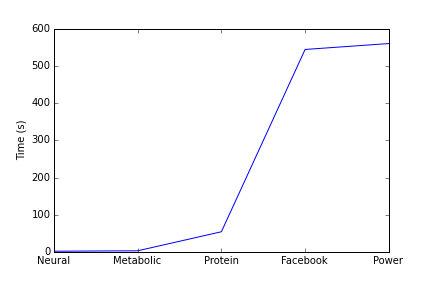
\includegraphics[width = \linewidth]{total.png}
\caption{Total solve time for each graph Laplacian linear system.}
\end{figure}

%\bibliographystyle{siam}
%\bibliography{mastersbib}

\end{document}